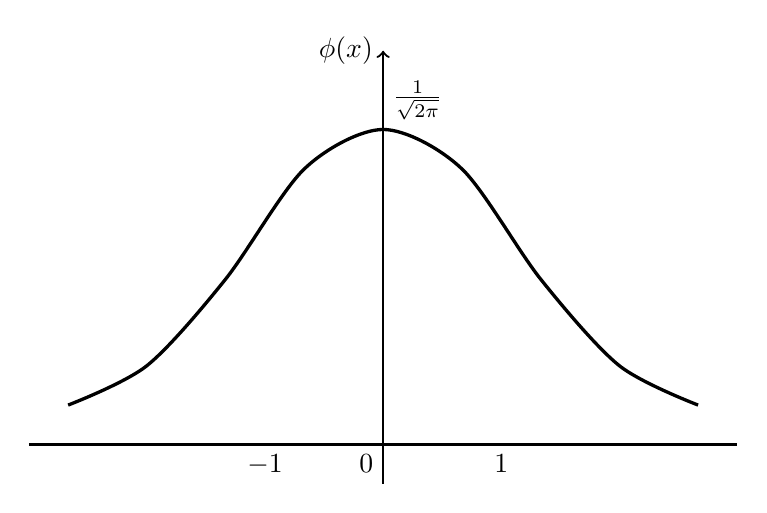
\begin{tikzpicture}
  \draw[->, thick] (4, -0.5) -- (4, 5)
    node[pos = 1, left] {\(\phi (x)\)};

  \draw (4, 4) node[above right] {\(\frac{1}{\sqrt{2 \pi}}\)};
  \draw (4, 0) node[below left] {\(0\)};

  \draw (2.5, 0) node[below] {\(-1\)};
  \draw (5.5, 0) node[below] {\(1\)};
  
  \draw[thick] (-0.5, 0) -- (8.5, 0);

  \draw[very thick]
    plot[smooth] coordinates {
      (0, 0.5) (1, 1) (2, 2.1) (3, 3.5) (4, 4)
      (5, 3.5) (6, 2.1) (7, 1) (8, 0.5)
    };
\end{tikzpicture}